\chapter{RISC-V微译器设计与实现}\label{chap:RISC-V}

x86微译器借鉴x86处理器微码缓存的设计思路,
实现了一种高效的、软硬协同的、x86-to-x86的二进制翻译器,并通过翻译缓存消除了间接跳转的开销,
达到了较高性能。
但目前x86微译器只能支持x86指令集,无法支持其他指令集,而本文的主要工作是为了支持RISC-V指令集,
验证其对多指令集的支持能力,同时为未来支持更多指令集打下基础,
最终实现在单一硬件平台上实现多指令集的共存,并尽可能地接近原生执行效率。

本节主要讲解为了让\textbf{x86微译器}支持RISC-V架构需要做的工作,主要包括RISC-V指令集的支持、RISC-V ABI的支持等。
% 首先需要讲解\textbf{融合微码}的编码方式,是如何做到高可扩展性的。

\begin{figure}[!htbp]
  \centering
  \includegraphics[width=0.8\linewidth]{./image/front_end_RISCV.pdf}
  \bicaption{\enspace RISC-V微译器整体架构图}{\enspace The overview of the RISC-V micro-translator architecture}
  \fignote{绿色部分为本文重点工作,在x86微译器上支持RISC-V架构所需要的修改。}
  \label{img:front_end_riscv}
\end{figure}

如图\ref{img:front_end_riscv}讲解了在x86微译器上添加RISC-V架构所需要的修改,其中绿色部分为本文主要工作,
包括软件层添加RISC-V二进制翻译器,硬件层添加对应的融合微码指令并在后端执行单元添加对应的执行逻辑。

\section{软件层RISC-V二进制翻译器}

本文首先重构了微译器中软件层二进制翻译器的代码,使其支持如下3个设计目标:
\begin{enumerate}
  \item 可扩展性强:能够方便支持多种指令集的翻译。
  \item 代码发现性强:能够发现更多的二进制代码进行翻译,减少动态二进制翻译的介入。
  \item 可维护性强:能够方便的维护和更新翻译器。
\end{enumerate}

\begin{figure}[!htbp]
  \centering
  \includegraphics[width=1\linewidth]{./image/mut_bt.pdf}
  \bicaption{\enspace 静态二进制翻译器架构图}{\enspace The architecture of the static binary translator}
  \label{img:mut_bt}
\end{figure}

因此在实现上,如图\ref{img:mut_bt},尽可能的将翻译器的功能模块化,分为代码发现模块、反汇编模块、翻译模块、提交模块。
代码发现模块用于尽可能的发现更多的二进制代码,例如通过符号表、字符串表等信息发现更多的代码;
反汇编模块用于将ELF文件中的二进制代码转换为汇编代码;
翻译模块用于将汇编代码翻译为融合微码指令;
提交模块用于将翻译后的融合微码指令组织成翻译缓存行的形式,写入预翻译文件。

此外将架构相关的代码和架构无关的代码分开,架构相关的代码只有翻译模块,架构无关的代码主要是代码发现模块、反汇编模块和提交模块。
这样只需要添加新的翻译模块,就能够支持新的指令集的翻译,而不需要修改其他模块的代码。

最后会希望尽可能复用现有的工具,例如LLVM objdump工具用于代码发现,这样能够减少二进制翻译器的实现难度,提高开发效率;
使用capstone工具用于反汇编,这样能够减少反汇编的实现难度,提高反汇编的准确性。
此外选用的LLVM objdump 和capstone工具都天然支持多种指令集,这样能够方便未来支持多种指令集的翻译。


% 而对于动态二进制翻译器,它的基本功能是在翻译缓存未命中时实时翻译客户指令,它和静态二进制翻译器的功能类似,
% 只是触发时机不同,因此我们可以复用静态二进制翻译器的代码,只需要添加一个触发机制即可。
% 它有两个触发机制,一个是代码发现没有发现的代码,需要实时翻译;一个是由于自修改代码等原因,翻译缓存行失效,需要实时翻译。
% 具体在硬件上,当翻译缓存行失效时,会触发例外(类似缺页异常),这时会调用动态二进制翻译器进行实时翻译,将翻译结果写入翻译缓存。


\section{融合微码设计}

本节详细介绍重要的一个概念——融合微码。“融合”代表它能融合了多种指令集的特征,
包括x86和RISC-V,未来还可以支持ARM,MIPS等其他指令集,
或许叫统一微码也更好理解。但融合并非简单的把所有指令集简单拼接就好,这会造成指令集冗余,挤占有限的编码空间。
而是需要对各个指令集的特征进行分析,找到共性,抽象出一种更加简洁的指令集,这就是融合微码的设计思想。

对于RISC-V微译器而言,融合微码是在前文\ref{sec:tisa}节中x86微码指令集进行扩充得到的。
本节首先讲解\textbf{融合微码}的编码方式,
通过调整融合微码的编码方式,使得微码能够支持多种指令集的翻译,同时保持简洁性、可扩展性。

\begin{figure}[!htbp]
  \centering
  \includegraphics[width=0.8\linewidth]{./image/TISA_encoder.pdf}
  \bicaption{\enspace 融合微码编码方式}{\enspace The encoding of the fused microcode}
  \label{img:TISA_encoder}
\end{figure}

融合微码的设计准则是需要高效的支持多种指令集,并且保持精简指令集(RISC)的特点。
它的目标是同时支持x86、RISC-V、ARM等多种指令集,而这些指令集的编码方式差异较大,
例如x86是变长指令集,长度可以从1字节到15字节不等,而RISC-V、ARM是固定长度指令集,长度为4字节;
不同指令集的寄存器数量、立即数长度、指令格式等也有很大差异;
对于同一个立即数,可能存储在不同的位置,例如RISC-V的12位立即数会根据不同的指令格式存储在不同的位置,可能分散存储在指令开头和中间。
融合微码希望屏蔽这些差异,尽可能简洁,同时保持高效。

此外,参考RISC-V 中压缩指令集的特点,本文将融合微码指令尽可能编码为2字节,
以减少一条融合微码的占用空间,提高一行翻译缓存行中微码数量,提高翻译缓存的命中率,提高性能。
因此融合微码指令同时支持2字节和4字节编码,如图\ref{img:TISA_encoder}所示,
前4行为4字节编码,后3行为2字节编码,后文默认把4字节编码指令称为\textbf{标准指令},2字节编码指令称为\textbf{压缩指令},
根据指令最低位是否为0来区分。

如图\ref{img:TISA_encoder},展示了融合微码的编码方式,主要包括两部分:操作码、操作数;其中操作数又分为立即数、寄存器、操作数长度。



\subsection{操作码}
对于操作码,按照操作数的数量分为0、1、2、3、4个操作数,对应的操作码(opcode)为opc0、opc1、opc2、opc3、opc4。
其中opc4、opc3只能在标准指令中使用,因为压缩指令只有2字节,不足以存储4个操作数的信息。
而opc0只能在压缩指令中使用,不需要存储操作数信息。
而opc1、opc2可以在标准指令和压缩指令中都可以使用,按照后缀区分为opc1f、opc1c、opc2f、opc2c,f后缀表示标准指令,c后缀表示压缩指令。

根据编码槽位可知,对于标准指令:opc4指令支持256个操作码,opc3指令支持8160个操作码,opc2f指令支持1008个操作码,opc1f指令支持512个操作码;
对于压缩指令:opc2c指令支持31个操作码,opc1c指令支持31个操作码,opc0指令支持32个操作码。
可见标准指令的编码空间更大,支持更多的操作码,而压缩指令的编码空间较小,只支持少量操作码,需要谨慎选择更常用的指令作为压缩指令。

\subsection{操作数长度}
对于操作数长度,按照操作数的长度分为1、2、4、8个字节,分别对应8位、16位、32位、64位操作数,这需要2比特来编码,存放在标准指令的最高位(sz位,size)。
对于压缩指令,由于编码空间很有限,需要的操作数长度只能编码在操作码(opc)中。
这主要是为了支持x86指令,由于历史原因,x86支持了多种操作数长度,例如add指令支持8位、16位、32位、64位操作数;
而现在的精简指令集,一般只支持固定长度的操作数,例如RISC-V的指令集,只支持32位和64位操作数,分别使用addw和add指令。

操作数长度本质上也可以看做操作码(opc)的一部分,放在指令最高位只是为了方便解码,减少解码的复杂度。
但在后续实现中发现可能不同的操作数会使用不同的长度,例如opc4指令中的第一个操作数可能是4字节,第二个操作数可能是2字节,那么这时候的sz位就没有作用了,
因此本文的设计中,sz位只是一个辅助位,如果操作数长度不同,需要在操作数的编码中明确指定。
% 所以在这种情况下,我们发现sz位的作用不大,因此后续的设计中可能会去掉sz位,统一放到操作数的编码中。

\subsection{立即数}

目前所有指令集都会把立即数编码在指令中,但由于x86是变长指令集,x86最多支持64位立即数,32位的偏移量(Displacement);
而RISC-V最多支持12位和20位立即数,AArch64支持12位和16位立即数,并且都没有偏移量的概念。
因此融合微码需要支持多种立即数的编码方式,同时保持简洁性。

% 如图\ref{img:immsize_x86}展示了x86的立即数和地址偏移的分布,
% 可以看到接近10\%的指令都使用了超过12位的立即数(注意并不是每一条指令都会用到立即数和地址偏移,所以指令总和不是100\%),
% 而地址偏移分布也比较分散,接近2\%指令使用了超过20位的地址偏移。
对于图\ref{img:immsize_riscv}展示了RISC-V的立即数分布(包含了访存指令的地址偏移),同样发现接近10\%的指令使用了接近12位的立即数。
如果直接将12位立即数直接编码到融合微码中,会导致编码空间不够,难以支持多种指令集、多种立即数的编码方式。

% \begin{figure}[h]
%   \centering
%   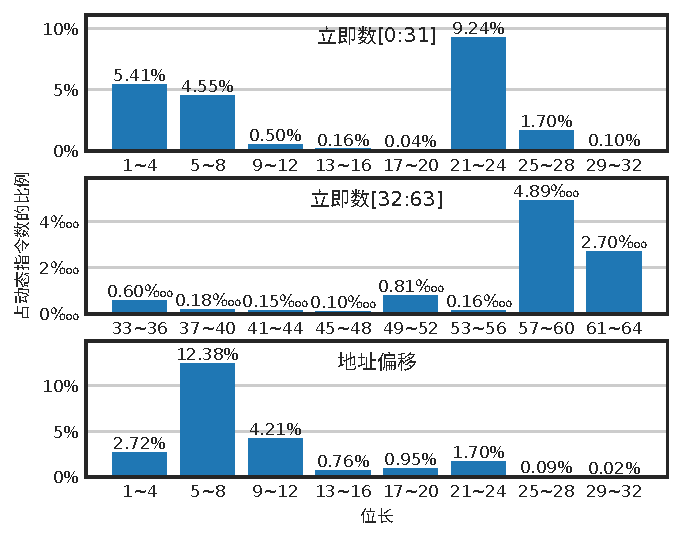
\includegraphics[width=0.8\linewidth]{./plot_pdf/immsize_x86.pdf}
%   \bicaption{\enspace x86 SPEC2017 中立即数和地址偏移的分布}{\enspace The immediate and displacement Distribution in x86 SPEC2017}
%   \label{img:immsize_x86}
% \end{figure}

\begin{figure}[h]
  \centering
  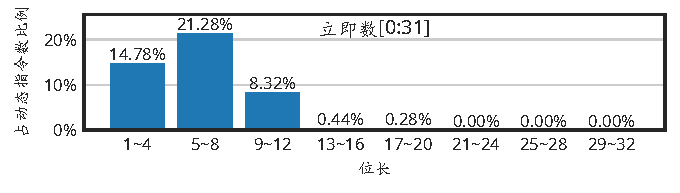
\includegraphics[width=0.8\linewidth]{./plot_pdf/immsize_riscv.pdf}
  \bicaption{\enspace RISC-V SPEC2017 中立即数分布}{\enspace The immediate Distribution in RISC-V SPEC2017}
  \label{img:immsize_riscv}
\end{figure}

因此参考微码缓存的设计思路,将短的立即数直接编码在操作数中,长的立即数存储在微码缓存行的立即数区域。
由于指令编码空间有限,并且出于简洁性的考虑,只把4比特以下的立即数编码在操作数中,更长的立即数存储在立即数区域,
前者称为\textbf{直接立即数},后者称为\textbf{间接立即数},用5比特的操作数(opr)最高位来区分;
如果为0,表示直接立即数,把短立即数直接编码在操作数中;如果为1,表示间接立即数,把长立即数的长度(len)编码在操作数中,
而真正的立即数需要根据立即数的索引到立即数区域中查找。
存储立即数长度(len)是为了支持\textbf{变长立即数},例如0x1ff,需要2字节来存储,而0x1ff00,需要3字节来存储,
这样可以根据len来到立即数区域中取出对应长度的立即数,
并不需要每个立即数都使用4字节存储,而是按需存储,节省编码空间。


\subsection{寄存器}

目前主流指令集都支持的通用寄存器数量不同,例如x86有16个通用寄存器,RISC-V和AArch64有32个通用寄存器。
过少的通用寄存器数量会导致寄存器分配困难,会溢出到内存中,增加访存开销;
过多的通用寄存器数量会导致更多的寄存器编码,增加编码空间,因此在设计中,只支持32个通用寄存器的编码,通过5比特的操作数(opr,operand)来寻址寄存器。

由于翻译器还需要使用一些临时寄存器,例如用于存储中间结果的寄存器,对于32个通用寄存器可能不够用,因此还需要支持\textbf{临时寄存器},
临时寄存器类似于x86的段寄存器或者RISC-V的CSR寄存器,只能用于存储临时数据,不能用于通用寄存器的操作。
所以还需要添加一些搬运指令,用于临时寄存器和通用寄存器之间的数据搬运。

对于浮点寄存器,目前主流指令集都是使用单独的浮点寄存器(X87 会使用浮点栈,本文并不支持,目前gcc编译生成的代码也基本不会使用X87),
例如x86 SSE指令集有16个128位的XMM寄存器,
RISC-V有32个64位的浮点寄存器。综合考虑,在设计中,只支持32个64位浮点寄存器的编码,同样通过5比特的操作数(opr)来寻址浮点寄存器。

如图\ref{img:regs},展示了融合微码的寄存器编码方式,主要包括通用寄存器、浮点寄存器和临时寄存器。

\begin{figure}[h]
  \centering
  \includegraphics[width=0.8\linewidth]{./image/regs.pdf}
  \bicaption{\enspace 微译器寄存器设计}{\enspace The design of the micro-translator registers}
  \label{img:regs}
\end{figure}



\section{RISC-V指令翻译}

上节中的融合微码编码设计是支持多种指令集的基础,本节主要介绍RISC-V指令和x86指令的语义差异,
以及如何通过添加微码指令来支持RISC-V指令的高效翻译。

设计一套高效完备的融合微码“指令集”是一个长期的工程,这不是本文研究重点。
为了快速验证微译器的实际效果,同时减少“指令集设计”产生的额外性能影响,
因此目前的融合微码是基于原本的\textbf{Gem5 x86微码}上\textbf{扩充}的,
基于这种扩充的方式,所有x86指令都可以直接翻译成一条或者多条融合微码指令,而RISC-V指令的翻译则
需要分析RISC-V指令和x86指令(x86微码)的语义差异,然后添加新的融合微码指令。

如图\ref{img:TISA},由于x86指令默认符号扩展,而RISC-V指令同时支持符号扩展和零扩展,
为了尽可能实现一条RISC-V指令翻译成一条融合微码指令,所以需要添加适当的“零扩展”微码指令。

\begin{figure}[!htbp]
  \centering
  \includegraphics[width=1\linewidth]{./image/TISA.pdf}
  \bicaption{\enspace 指令翻译到融合微码过程}{\enspace The process of translating instructions to fused microcode}
  \fignote{x86 add 和RISC-V add 指令都翻译成融合微码add指令,
  而lbu(加载字节并无符合扩展)指令,需要额外添加lbu 微码指令。}
  \label{img:TISA}
\end{figure}

融合微码添加有两大设计原则:
\begin{enumerate}
  \item \textbf{一对一原则}: 一条RISC-V指令尽可能翻译成一条融合微码指令,减少指令翻译的膨胀率,提高性能。
  \item \textbf{复用原则}: 尽可能复用现有的x86微码,减少硬件侧新指令的添加,减少硬件开发的复杂度。
\end{enumerate}

目前已经完成所有的RISC-V指令(包括IMAFDC指令集,简称GC指令集)到融合微码的翻译,完整的翻译表格见附录\ref{app:RISC-V}。

不同类别的指令翻译如下:

\subsection{整数指令}
整数指令(I)主要包括移位指令、算数指令、逻辑指令、比较指令、分支指令、访存指令等。
大部分复用x86微码,例如加法add指令复用x86的addflags指令(会计算EFLAGS,但RISC-V不会使用它);
其余的无法一对一翻译的指令,需要添加新的微码指令。

例如对于大多以w结尾的指令,例如addw指令,这是RISC-V64位指令集中的32位加法指令,默认进行符号扩展并填入64位寄存器,
而x86微码中没有这种指令,所以需要添加一个addw微码指令。而对于auipc指令,这是RISC-V中的一个特有指令,需要添加一个auipc微码指令。
访存指令中的lb、lh、lw、lbu、lhu指令,这些指令需要额外添加微码指令,用于加载字节、半字、字,并进行符号扩展或者零扩展。

此外,翻译出的指令还需要利用到硬件原有特性,例如x86的call 和ret 指令会利用硬件返回栈(return stack,RAS),用于把返回地址压栈,
并在ret指令中弹栈,这样可以减少分支预测错误率。
而RISC-V会使用jal、jalr指令来作为函数调用和返回,所以需要添加jal\_call、jalr\_ret微码指令,并充分利用硬件的返回栈机制。


\subsection{乘除法指令}
乘除法指令(M)主要包括乘法、除法、取余等指令。
对于32位乘法,RISC-V指令默认需要2条指令才能得到完整的64位乘法结果,而x86微码中默认只用了1条微码,
所以对于这类乘除法指令,需要添加新的微码指令。以w结尾的指令,例如mulw指令,默认进行符号扩展并填入64位寄存器,也需要添加新的微码指令。

\subsection{原子指令}
原子指令(A)包括原子加法、原子比较等指令。由于目前尚未实现多线程支持,使用普通的指令替代原子指令,暂时没有考虑原子性问题。
如图\ref{img:amo_trans}展示了一条原子加法指令的翻译过程,会翻译成6条融合微码指令。
这也是唯一出现的一类RISC-V指令翻译成了多条融合微码指令,其余指令都是一条指令翻译成一条融合微码指令。
但由于原子指令出现的频率极低,在单线程情况下对性能影响不大。

\begin{figure}[!htbp]
  \centering
  \includegraphics[width=0.6\linewidth]{./image/amo_trans.pdf}
  \bicaption{\enspace RISC-V原子加法指令翻译过程}{\enspace The translation process of RISC-V atomic addition instruction}
  \fignote{会使用两个临时寄存器,需要前后都进行寄存器保存和寄存器恢复。
  暂未实现多线程,没有考虑原子性问题。}
  \label{img:amo_trans}
\end{figure}

\subsection{浮点指令}
浮点指令(F,D)包括单精度浮点F 和双精度浮点D指令。
由于x86 SSE模式下的浮点指令和RISC-V浮点指令都遵循IEEE-754标准,所以很多可以直接复用x86的浮点微码指令。
出于简洁考虑,对于特殊的舍入模式暂未考虑和x86的差异,对于运行SPEC CPU 2000中的浮点测试,没有发现问题。

此外,x86 SSE模式下使用16个128位的XMM寄存器,用于存储浮点和整数,
而RISC-V使用32个专用的64位的浮点寄存器,
微译器使用32个64位浮点寄存器并直接复用x86的浮点微码指令。
而对于RISC-V的浮点寄存器和通用寄存器之间的数据搬运,x86没有这种指令,
所以需要添加新的浮点寄存器搬运指令,
用于浮点寄存器和通用寄存器之间的数据搬运。
对于浮点转换指令,例如fcvt.w.s指令,这是RISC-V中的一个特有指令,需要添加一个fcvt.w.s微码指令。

\subsection{压缩指令}
压缩指令(C):为了压缩指令长度,把常用的4字节指令替换为2字节长度的压缩指令。
会尽可能把原本就是2字节的RISC-V压缩指令直接翻译成2字节的融合微码指令,
例如c.add指令翻译为c\_add微码指令。



\subsection{小结}

累积统计数目如下:原本x86指令共有数千条,x86微码也有500余条。
为了添加272条RISC-V指令,本文并没有简单添加272条微码指令,
而只是添加了41条整数相关指令,10条浮点相关指令,累计添加51条微码指令。
如图\ref{img:isa_num}展示了指令翻译的数量统计。


\begin{figure}[!htbp]
  \centering
  \includegraphics[width=0.7\linewidth]{./image/isa_num.pdf}
  \bicaption{\enspace x86、RISC-V指令翻译到融合微码的数目统计}{\enspace The number of x86 and RISC-V instructions translated to fused microcode}
  \label{img:isa_num}
\end{figure}

\section{硬件层执行单元修改}

本节主要介绍硬件层的修改,由于添加了新的融合微码指令,需要修改硬件层的微码执行单元,使其能够支持新的融合微码指令。
由于本文在Gem5模拟器的基础上进行修改,因此只需关注指令的功能实现以及一条指令的执行周期数。

本文添加的融合微码指令和原有的x86微码相比,功能上没有太大的区别,主要是添加了一些新的指令,例如lbu、addw、auipc等,
这些指令都能在硬件层找到对应的功能单元,只需要修改微码执行单元的控制逻辑即可,并且可以在一个周期内完成。
而对于乘法、除法指令,和原本x86微码一样,默认进入对应的乘法、除法功能单元,分别需要多个周期完成。


\section{RISC-V ABI差异处理}
%介绍什么是ABI, 从而引出RISC-V和x86的ABI差异。而我们的项目需要把RISC-V的ABI转换成x86的ABI。
ABI全称为Aplication Binary Interface(应用二进制接口),
为程序提供了一种与操作系统和硬件交互的接口,定义了程序的二进制接口,包括数据类型、函数调用约定、系统调用等内容。
不同指令集的ABI也是不同的,
在二进制翻译系统中需要维护这种差异性,保证程序运行的正确性。
ABI包括内容比较多,其中主要的包括系统调用传参、初始化栈等问题,本节介绍RISC-V微译器项目是如何处理ABI差异的。


\subsection{系统调用差异}

如表\ref{tab:syscall}所示,总结了x86和RISC-V的系统调用号和参数传递方式的差异。
x86的系统调用号存储在rax寄存器中,返回值也存储在rax寄存器中,参数传递方式为rdi, rsi, rdx, r10, r8, r9。
而RISC-V的系统调用号存储在a7寄存器中,返回值存储在a0寄存器中,参数传递方式为a0, a1, a2, a3, a4, a5。
因此需要在RISC-V的二进制翻译器中,将RISC-V的系统调用号和参数传递方式转换成x86的系统调用号和参数传递方式。

参数传递的差异可以通过把x86的参数寄存器和RISC-V的参数寄存器映射到相同的微码寄存器即可,如表\ref{tab:reg_map}所示,
所有的黄色寄存器就是6个参数传递寄存器。系统调用号差异同理也可解决。



\begin{table}[h]
    \centering
    \footnotesize% fontsize
    \setlength{\tabcolsep}{4pt}% column separation
    \renewcommand{\arraystretch}{1.2}%row space 
    % \begin{adjustbox}{width=\textwidth}
      \begin{tabular}{llllllllll}
      \hline
      指令集 & 系统调用号 & 返回值 & 参数1 & 参数2 & 参数3 & 参数4 & 参数5 & 参数6 & 其他参数 \\ \hline
      x86     & rax    & rax   & rdi & rsi & rdx & r10 & r8  & r9  & 栈传递  \\
      RISC-V  & a7     & a0    & a0  & a1  & a2  & a3  & a4  & a5  & 栈传递 \\
      \hline
      \end{tabular}
    % \end{adjustbox}
    \bicaption{\enspace x86和RISC-V的系统调用差异}{\enspace The difference between x86 and RISC-V system calls}
    \label{tab:syscall}
  \end{table}
  

\subsection{寄存器映射}

寄存器映射一直是二进制翻译中一个重要的研究课题。
如表\ref{tab:reg_map}所示,展示了x86和RISC-V映射到微码的的寄存器映射表。
对于x86寄存器映射到微码寄存器较为容易,因为x86只有16个通用整数寄存器,而微码定义了32个通用寄存器,
所以只需要把x86寄存器固定映射到前16个通用寄存器即可,还可以把一些常用的寄存器
(例如AH,BH等子寄存器和段寄存器)映射到后面的寄存器中,剩余的一些寄存器作为临时寄存器供二进制翻译器使用。

\begin{table}[!htbp]
  \centering
  \bicaption{\enspace x86和RISC-V到微码的寄存器映射表}{\enspace The register mapping table from x86 and RISC-V to microcode}
  \label{tab:reg_map}
  \footnotesize% fontsize
  \setlength{\tabcolsep}{4pt}% column separation
  \renewcommand{\arraystretch}{1.2}%row space 
  % \begin{adjustbox}{width=\textwidth}
      \begin{tabular}{lll|lll|lll|lll}
  \hline
  微码                        & x86                         & RISC-V                     & 微码                         & x86                         & RISC-V                     & 微码 & x86 & RISC-V & 微码 & x86 & RISC-V \\ \hline
  \cellcolor[HTML]{FFCC67}0 & \cellcolor[HTML]{FFCC67}RAX & \cellcolor[HTML]{FFCC67}A7 & \cellcolor[HTML]{FFCC67}8  & \cellcolor[HTML]{FFCC67}R8  & \cellcolor[HTML]{FFCC67}A4 & 16 & T0  & Zero   & 24 & T8  & S8     \\
  1                         & RCX                         & TP                         & \cellcolor[HTML]{FFCC67}9  & \cellcolor[HTML]{FFCC67}R9  & \cellcolor[HTML]{FFCC67}A5 & 17 & T1  & RA     & 25 & T9  & S9     \\
  \cellcolor[HTML]{FFCC67}2 & \cellcolor[HTML]{FFCC67}RDX & \cellcolor[HTML]{FFCC67}A2 & \cellcolor[HTML]{FFCC67}10 & \cellcolor[HTML]{FFCC67}R10 & \cellcolor[HTML]{FFCC67}A3 & 18 & T2  & S2     & 26 & T10 & S10    \\
  3                         & RBX                         & GP                         & 11                         & R11                         & A6                         & 19 & T3  & S3     & 27 & T11 & S11    \\
  4                         & RSP                         & SP                         & 12                         & R12                         & T1                         & 20 & T4  & S4     & 28 & T12 & T3     \\
  5                         & RBP                         & T0                         & 13                         & R13                         & T2                         & 21 & T5  & S5     & 29 & T13 & T4     \\
  \cellcolor[HTML]{FFCC67}6 & \cellcolor[HTML]{FFCC67}RSI & \cellcolor[HTML]{FFCC67}A1 & 14                         & R14                         & S0                         & 22 & T6  & S6     & 30 & T14 & T5     \\
  \cellcolor[HTML]{FFCC67}7 & \cellcolor[HTML]{FFCC67}RDI & \cellcolor[HTML]{FFCC67}A0 & 15                         & R15                         & S1                         & 23 & T7  & S7     & 31 & T15 & T6     \\ \hline
  \end{tabular}
  % \end{adjustbox}
\end{table}

但是对于RISC-V映射到微码方案,由于RISC-V本身就有32个通用寄存器,固定映射到32个微码寄存器后,
就没有额外的临时寄存器供二进制翻译器使用了。对于微译器项目,得益于软硬件协同设计的基本原则,
本文额外添加了两个微码寄存器作为临时寄存器,
这两个寄存器只对二进制翻译器可见,不对RISC-V应用程序可见,类似于x86“段寄存器”,属于特殊寄存器,具体的使用场景参考图\ref{img:amo_trans}。

此外,相对于传统的软件二进制翻译器,
微译器不需要维护源寄存器块、源内存镜像等信息,不需要管理代码缓存,
因此可以减少翻译器由于翻译机制占用的寄存器数量,降低寄存器压力。


\subsection{栈的初始化}
由于我们目前关注于用户态二进制翻译器,不太涉及系统态指令的翻译和处理操作系统等概念,
但是当加载运行不同指令集的程序时,在libc库眼中,操作系统已经准备好了这个程序的初始化栈等信息,例如argc,argv参数、
环境变量指针等,对于x86和RISC-V程序,这个初始化栈是不同的,需要不同的处理。

用户态模拟的Gem5模拟器,会扮演操作系统的角色,负责加载程序、初始化栈、运行程序等操作。
因此需要修改Gem5在启动RISC-V程序的初始化栈,把RISC-V相关的argc、argv、envp等信息放到正确的位置。

而对于真实处理器,需要在操作系统层面进行修改,把RISC-V的ABI转换成x86的ABI,
并修改加载器用以识别不同指令集的程序并初始化栈,
这是一个较为复杂的工作,不在本文的研究范围内。

\section{本章小结}

本章主要介绍了在微译器中添加RISC-V支持所需要的工作,包括软硬件层的设计和修改。
首先把软件层二进制翻译器重构为适合多架构翻译的框架、将体系结构相关和无关的代码分离;
接下来讲解了融合微码的设计和实现,包括操作码、操作数长度、立即数、寄存器等的设计,如何更好的支持多种指令集;
然后介绍了RISC-V指令的翻译,主要是RISC-V和x86指令的语义差异,如何通过添加尽可能少的微码指令来支持RISC-V指令;
其次介绍了硬件层的修改,主要是添加新的融合微码指令对具体功能部件的修改;
最后介绍了RISC-V和x86的ABI差异,RISC-V微译器通过寄存器映射来处理系统调用差异、并处理了栈的初始化问题。